\chapter*{Leafletによるブラウザへの表示}

タイルサーバを作成したら、ブラウザへの表示を行ってみましょう。
GoogleMapのようにマウスでぐりぐり動く地図を作るためのJavaScriptライブラリが
すでに公開されています。
特に、OpenLayersとLeafletが二大巨塔です。今回はLeafletを使ってブラウザに表示してみます。

\section*{OpenStreetMapの表示}

まずは、ベースタイルとなる、OpenStreetMapを表示するJavaScriptを書いてみます。
OpenStreetMapを表示するだけなら簡単です。
Listing \ref{osm_html}と\ref{osm_js}にOSMを表示する
HTMLとJavaScriptを示します。Listing \ref{osm_js}のJavaScriptは、map.jsという
ファイル名で保存されているとします。

Listing \ref{osm_html}では、LeafletのCSSとScriptをCDNから読み込んでいるだけです。
CDNのURLやintegrityは、Leaflet Tutorial (http://leafletjs.com/examples/quick-start/)にあります。
HTMLのBODYにある、mapというIDが付いたDIV要素に地図が表示されます。
DIV要素は、デフォルトではサイズが0なので、Stylesheetで地図を表示するサイズを指定します。
これを忘れると、ちゃんと動いているのに表示されないとハマる事になります。
今回は、style属性に書いています。

\lstinputlisting[caption=OpenStreetMapの表示 (HTML),label=osm_html]{osm.html}

Listing \ref{osm_js}のスクリプトのほうは、Mapオブジェクトのインスタンスを作成して
OSMのタイルのURLを指定した、TyleLayerインスタンスを作成後、Mapインスタンスに追加しているだけです。
MapクラスのsetViewメソッドで地図の中心座標と、ズームレベルを指定しています。
この例では、北緯35.6299度、東経129.7919度、ズームレベル16を指定しています。
ビッグサイトのあたりが表示されるはずです。

\lstinputlisting[caption=OpenStreetMapの表示 (JavaScript),label=osm_js]{osm.js}

TileLayerクラスのコンストラクタにタイルのURLと、著作権情報を指定しています。
タイルのURLはすでに説明しました。
著作権情報は、OSMの場合は必須です。地理院地図でも同様です。
どのように記述するかは、各Webページをご覧ください。
\begin{itemize}
\item OpenStreetMap http://wiki.openstreetmap.org/wiki/JA:Legal\_FAQ
  \item 地理院地図 http://maps.gsi.go.jp/help/use.html
\end{itemize}

\section*{タイルのオーバーレイ}
      
では、これに今回作ったタイルを重ねましょう。
Listing \ref{osm_js}を見ればわかるように、tileLayerのインスタンスを作って、
mapにaddすれば良いでしょう。作成したタイルを重ねたものを表示するJavaScriptをListing \ref{tile_js}に示します。
違いは、10行目以降です。今回作成したタイルサーバは、TMS準拠ですので
OSMやGoogleMapと緯度が増える方向が異なります。
そこで、tileLayerのtmsパラメータにtrueを指定しなければならないことに注意してください。

\lstinputlisting[caption=タイルのオーバーレイ (JavaScript),label=tile_js]{tile.js}

作成したHTMLとJSをタイルサーバにデプロイすれば、
オーバーレイしたマップを図\ref{fig:browser}のように
表示することができます。
紙媒体だと、モノクロ印刷なので良くわからないと思います。
GitHubにカラーのPDFをアップロードしておきますので、そちらを
ご覧ください。
\texttt{https://github.com/chomy/DevelopmentOfTMS}

\begin{figure}[t]
\centering
\scalebox{0.8}{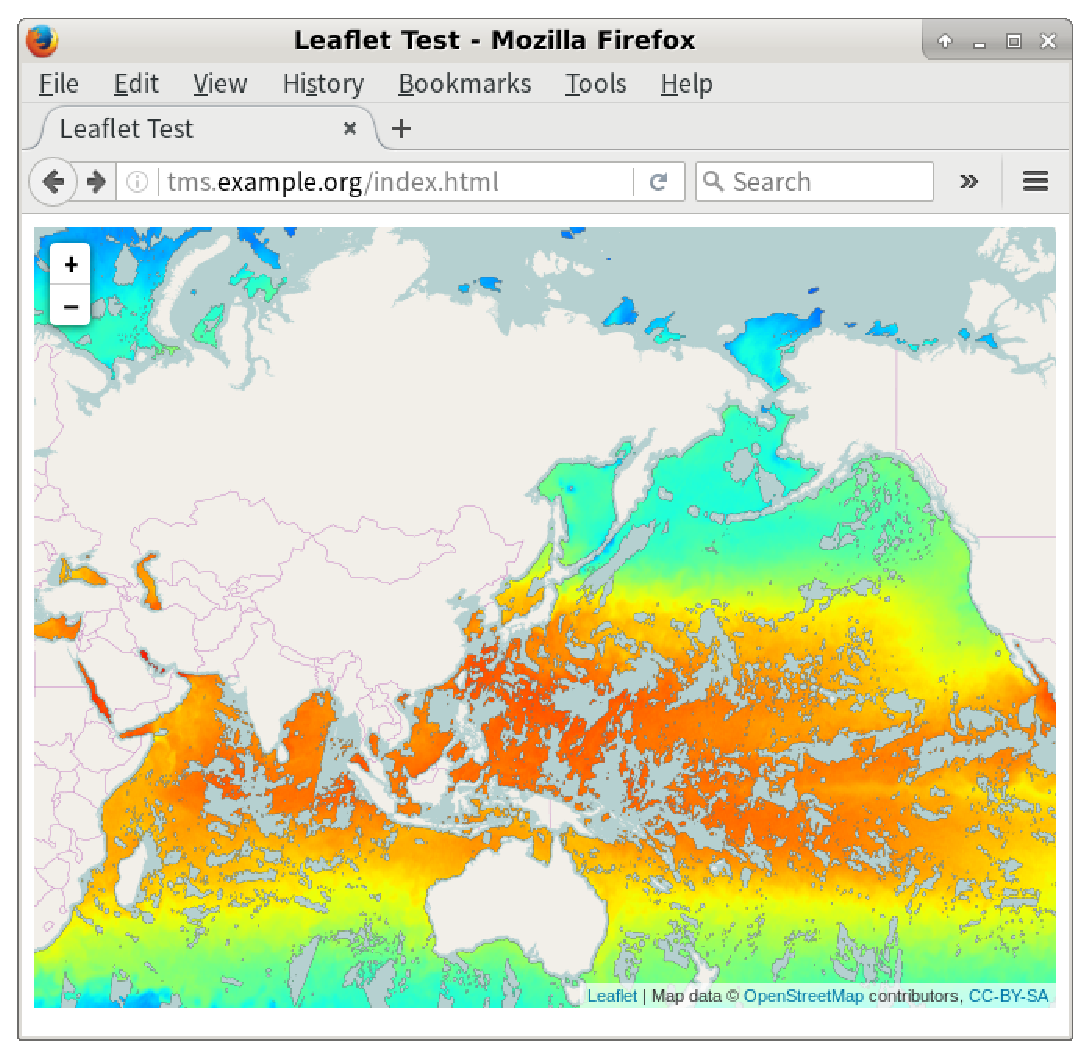
\includegraphics{browser.eps}}
\caption{ブラウザに表示したOpenStreetMapにオーバーレイした海水面温度の例}
\label{fig:browser}
\end{figure}


これで、地球観測衛星の観測データを可視化して、タイルとして
公開するタイルサーバが完成しました。
これは(細かい事は別にして)TMSに準拠したXYZタイルサーバですので
QGISといった、GISソフトはもちろん様々なサービスで使用することができます。
